\chapter{Přístrojové vybavení}
\label{sec:instruments}
Na úvod experimentální části je vhodné popsat konkrétní přístroje
a~další součásti používané při pokusech,
neboť některé se opakují ve více aparaturách.

\section{Laserová aparatura}
\label{sec:instruments-laser}

\subsection{Laser Ekspla \instrname{PL2231-50}}
\label{sec:instruments-laser-source}
Ústřední součástí všech prováděných pokusů byl samozřejmě laser.
Vždy bylo použito totéž zařízení, konkrétně model \instrname{PL2231-50}
od firmy Ekspla.
Je to diodou čerpaný pevnolátkový pikosekundový laser typu Nd:YAG
poskytující velmi krátké pulzy záření o~vysokém okamžitém výkonu.
Délka pulzu (FWHM) činí \SI{29}{\pico\second}
a~jejich energie může dosahovat až \SI{30}{\milli\joule},
což představuje okamžitý výkon v~řádu \si{\giga\watt}.
Pulzy se opakují s~frekvencí \SI{50}{\hertz}.

\begin{figure}[htp]
	\centering
	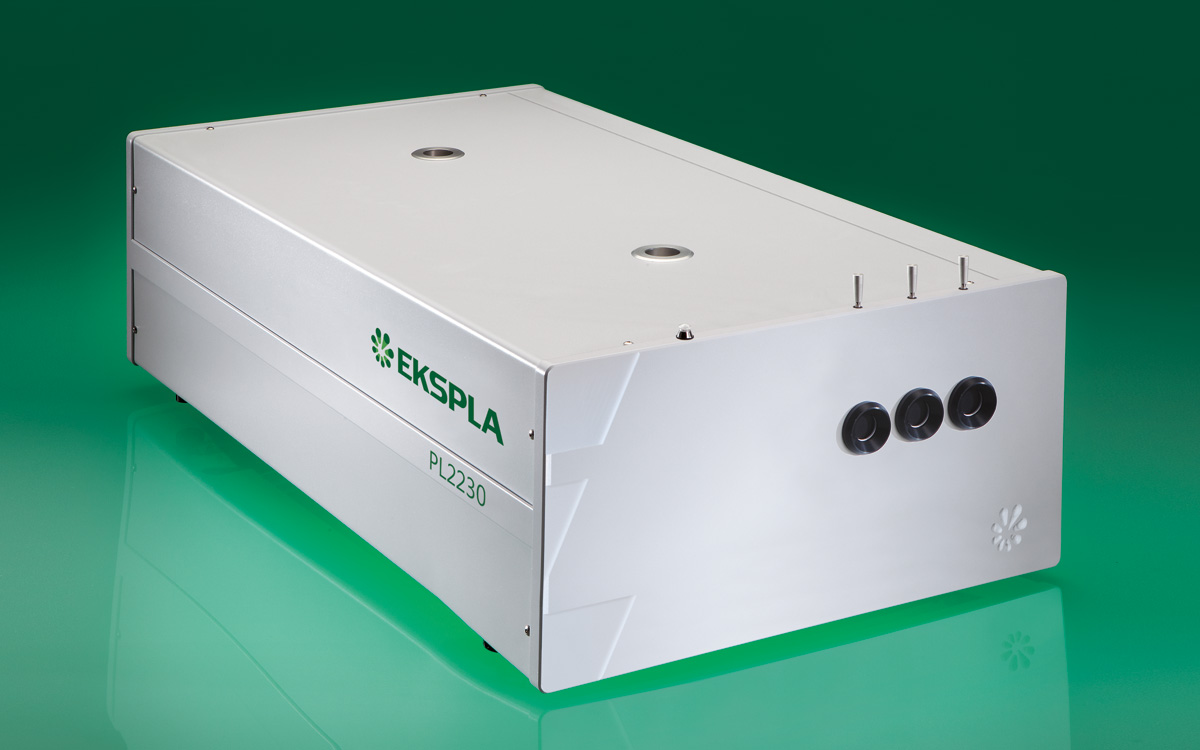
\includegraphics[width=\textwidth]{laser}
	\caption{Pikosekundový laser Ekspla (fotografie z~katalogu).
		Použitý model je ze stejné řady.
		Převzato z~\cite{ekspla-datasheet}.}
	\label{fig:instruments-laser}
\end{figure}

Aktivním médiem je krystal yttrito-hlinitého granátu (\ce{Y3Al5O12})
dopovaný ionty neodymu (\ce{Nd3+}).\autocite{wiki-ndyag}
Základní vlnová délka laseru je \SI{1064}{\nano\metre},
stejně jako pro všechny lasery typu Nd:YAG,
jeho součástí jsou ale teplotně stabilizované jednotky obsahující
krystaly di\-hydro\-gen\-fosfo\-rečnanu draselného (KDP a~KD*P),
které umožňují generování druhé a~třetí harmonické frekvence,
tedy vlnových délek \SIlist{532; 355}{\nano\metre}.
\autocite{ekspla-datasheet}

Generování začíná v~hlavním pevnolátkovém oscilátoru čerpaném diodami,
který vytváří řetězce pulzů s~frekvencí opakování jednotlivých pulzů
přibližně \SI{87}{\mega\hertz} (tzv.~\emph{trains}).
Pulzy jsou slabé, jejich energie se pohybuje v~jednotkách \si{\nano\joule}.
Tyto putují do diodového regenerativního zesilovače se zesílením v~řádu $10^6$
a~poté do víceprůchodového výkonového zesilovače,
takže jejich konečná energie je kolem $\SI{30}{\milli\joule}$.
Výstupní energie je nastavitelná v~krocích po zhruba \SI{1}{\percent}
a~je velmi stabilní mezi po sobě jdoucími pulzy
(odchylky jsou menší než \SI{0.5}{\percent} středního kvadratického průměru
při nastavené základní vlnové délce).
\autocite{ekspla-datasheet}

Výstupní svazek je z~\SI{99}{\percent} svisle polarizovaný.
Jeho profil je podle výrobce přibližně gaussovský
(viz obrázek~\ref{fig:instruments-beamprofile})
o~průměru cca \SI{6}{\milli\metre} na úrovni $1/e^2$ maxima
pro vlnovou délku \SI{1064}{\nano\metre}.
\autocite{ekspla-datasheet}

Laser je vybaven vlastním měřičem, který průběžně zaznamenává energii pulzu.
K~synchronizaci dalších zařízení slouží spouštěcí signál s~nastavitelným
předstihem.\autocite{ekspla-datasheet}

\begin{figure}[htp]
	\centering
	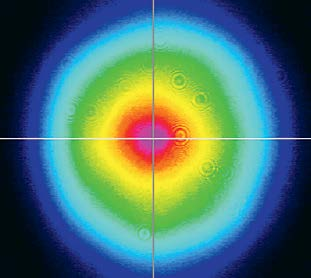
\includegraphics[scale=0.5]{ekspla-beamprofile}
	\caption{Typický profil laserového svazku pro \SI{1064}{\nano\metre}
		v~blízkém poli uvedený v~technickém listu laseru.
		Převzato z~\cite{ekspla-datasheet}.}
	\label{fig:instruments-beamprofile}
\end{figure}

\subsection{Optický zesilovač Ekspla \instrname{PG411-SH-DUV}}
\label{sec:instruments-laser-amp}
Součástí zdroje laserového záření je laditelný optický parametrický
zesilovač \instrname{PG411-SH-DUV} od téhož výrobce,
který produkuje intenzivní laserové pulzy s~laditelnou vlnovou délkou.

Zesilovač sestává ze dvou základních částí.
První je synchronně čerpaný optický parametrický oscilátor (SOPO),
který je čerpán sekvencemi pulzů o~četnosti přibližně \SI{87}{\mega\hertz}
a~vlnové délce záření \SI{355}{\nano\metre},
tedy třetí harmonické frekvenci laseru Nd:YAG.
Jeho výstupem je další sekvence pulzů pokračující do druhé části,
optického parametrického zesilovače (OPA).
Ten je čerpán jedním pulzem synchronizovaným s~výstupem SOPO.
Výsledkem je pak jeden vysokointenzitní pulz na pozadí sekvence slabých
pulzů o~rezonanční frekvenci parametrického oscilátoru,
v~ostatních frekvencích pozadí vymizí a je přítomen pouze hlavní pulz.
\autocite{ekspla-amp-datasheet}

Model \instrname{PG411} je optimalizován pro nejvyšší enegii pulzu
v~oblasti viditelného světla.
Sám o~sobě umožňuje ladění vlnových délek v~rozsahu
\SIrange{410}{2300}{\nano\metre},
ale navíc je vybaven generátorem druhé harmonické frekvence (SHG)
a~generátorem součtových frekvencí (DUV),
jež laditelný rozsah zvyšují na \SIrange{193}{2300}{\nano\metre}.

Nejvyšší opakovací frekvence pulzů je \SI{50}{\hertz}
a~maximální energie pulzu je \SI{50}{\micro\joule}.
Šířka čáry je nižší než \SI{3}{\per\centi\metre} ve středním rozsahu
(\SIrange{409}{710}{\nano\metre}),
v~ostatních oblastech nižší než \SI{5}{\per\centi\metre}.
Délka trvání pulzu je kolem \SI{20}{\pico\second}.
Výstupní svazek je svisle polarizovaný a~jeho průměr
jsou zhruba \SI{4}{\milli\metre}.
\autocite{ekspla-amp-datasheet}

\section{ICCD kamera \instrname{PI-MAX 1024}}
\label{sec:instruments-iccd}
Pro obrazový záznam rychlých dějů s~malou intenzitou záření byla použita
intenzifikovaná CCD kamera (ICCD) od Princeton Instruments.
Šlo o~zakázkově upravený model \instrname{PI-MAX 1024RB-25-FG-43}
se zmenšeným intenzifikátorem pro kratší integrační časy.

Snímačem kamery je CCD čip s~rozlišením \num{1024}\times\SI{256}{\pixel}.
Před snímačem je umístěn intenzifikátor \instrname{Gen II RB},
který je s~čipem spojen prostřednictvím svazku optických vláken.
Intenzifikátor typu \instrname{RB} má široký spektrální rozsah
od přibližně \SI{200}{\nano\metre} do \SI{900}{\nano\metre}
(viz obrázek \ref{fig:instruments-cameraeff}).

Intenzifikátor je zepředu chráněn křemenným vstupním sklem,
za nímž se nachází alkalická fotokatoda.
Jádrem intenzifikátoru je mikrokanálová destička,
která funguje jako fotonásobič každého kanálu
(jeden kanál odpovídá jednomu pixelu na čipu).
Pracovní napětí je kolem \SI{200}{\volt}.
Na vnitřní straně destičky je luminofor P43,
který znásobené elektrony převádí zpět na fotony,
jež putují svazkem optických vláken do CCD čipu.
\autocite{pi-iccd}
Čip je vybaven termoelektrickým chlazením pro potlačení temného proudu.
\autocite{pimax-datasheet}

Kamera umožňuje velmi krátké integrační časy pod \SI{2}{\nano\second}
a~záznam obrazu v~dlouhodobě udržitelné frekvenci 50 snímků za sekundu.
Časování je zajištěno vestavěným programovatelným generátorem \instrname{PTG}.
\autocite{pimax-datasheet}

\begin{figure}[htp]
	\centering
	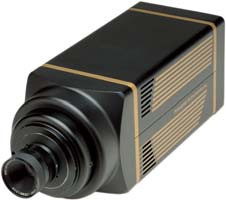
\includegraphics[scale=0.4]{img/pimax-1024}
	\caption{Intenzifikovaná CCD kamera \instrname{PI-MAX 1024}
		(fotografie z~katalogu).
		Převzato z~\cite{pimax-datasheet}.}
	\label{fig:instruments-camera}
\end{figure}

\begin{figure}[htp]
	\centering
	\input{img/cameraeff}
	\caption{Kvantová účinnost kamery deklarovaná výrobcem.
		Podle \cite{pimax-datasheet}.}
	\label{fig:instruments-cameraeff}
\end{figure}

Pro odstínění laserového světla byly v~některých pokusech využity dvě
křemenné destičky umístěné před objektivem kamery.
Jejich naměřená propustnost je na obrázku~\ref{fig:instruments-camerafilter}.

\begin{figure}[htp]
	\centering
	\input{img/camerafilter}
	\caption{Propustnost dvou křemenných skel sloužících jako filtr
		před kamerou.}
	\label{fig:instruments-camerafilter}
\end{figure}

Na rozdíl od prvního laseru výrobce nezaručuje prostorový profil
laserového svazku.
Při pokusech se ukázalo, že profil svazku je závislý
na nastavené energii pulzu v~míře, kterou nelze zanedbat.
Částečné nápravy tohoto stavu bylo dosaženo použitím prostorového filtru
(viz oddíl~\ref{sec:instruments-spatialfilter}).
Tato problematika je podrobněji popsána v~dalších kapitolách,
viz především oddíl \ref{sec:lif-rayleigh}.

\section{Měřiče energie Ophir}
\label{sec:instruments-powermeter}
K~měření energie laserového svazku sloužily pyroelektrické měřiče energie
od firmy Ophir.
Byly použity modely \instrname{PE9-SH-ROHS} a~\instrname{PE9-ES-C}.
Oba jsou vybaveny kovovým absorbérem se spektrálním rozsahem
\SIrange{0.15}{12}{\micro\metre}
a~opakovací frekvencí až \SI{25}{\kilo\hertz}.
Apertura přístroje je $\SI{8}{\milli\metre}$
a~maximální délka pulzu je $\SI{20}{\micro\second}$.
\autocites{pe9-datasheet,pe9esc-datasheet}
Měřitelný rozsah energií pulzu je \SIrange{0.2}{1000}{\micro\joule}
v~případě \instrname{PE9-SH-ROHS}\autocite{pe9-datasheet}
a~\SIrange{0.1}{200}{\micro\joule} v~případě \instrname{PE9-ES-C}
\autocite{pe9esc-datasheet}.

\begin{figure}[htp]
	\centering
	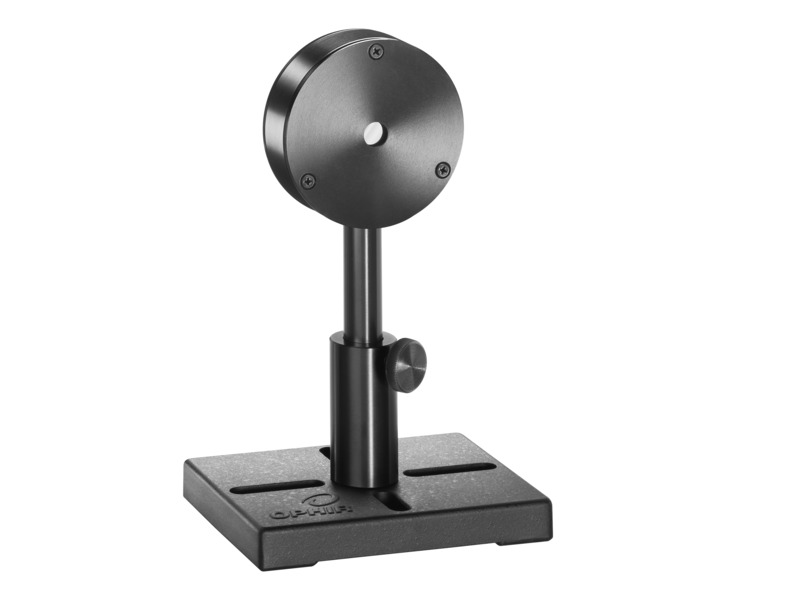
\includegraphics[width=0.5\textwidth]{img/ophir-pe9esc}
	\caption{Pyroelektrický měřič energie \instrname{PE9-ES-C}.
		Převzato z~\cite{pe9esc-datasheet}.}
	\label{fig:instruments-powermeter}
\end{figure}

\section{Prostorový filtr}
\label{sec:instruments-spatialfilter}
Méně běžným optickým prvkem, který se v~některých aparaturách vyskytoval,
byl takzvaný prostorový filtr.
To je zařízení, které umožňuje upravit prostorový profil laserového svazku
do vhodnější podoby, což nejčastěji znamená odstranit náhodné fluktuace,
aby se lépe podobal gaussovskému.

Tato nutnost vyplynula z~měření TALIF kryptonu (v~práci neuvedeného).
Bez prostorového filtru byla intenzita fluorescence výrazně ovlivňována
nestabilitou prostorového profilu intenzity laserového svazku.

Základní myšlenka prostorového filtru je jednoduchá:
Vytvořit fourierovský obraz původního svazku,
z~něj odfiltrovat nežádoucí prostorové frekvence
a~svazek rekonstruovat.
V~praxi se obvykle realizuje pomocí dvou spojek nebo jiných spojných soustav,
které jsou umístěny na ose svazku tak, že jejich ohniska mezi nimi splývají.
Ve~společné ohniskové rovině je clonka s~malým kruhovým otvorem,
která propouští jen středovou část obrazu (Airyho disk)
a~ořezává vyšší prostorové frekvence.
Při vhodně zvolené apertuře je možné takto za filtrem získat přibližně
gaussovský svazek.

Použitý prostorový filtr byl sestaven ze dvou křemenných spojek
s~ohniskovou vzdáleností \SIlist{10;20}{\milli\metre}.
